\chapter{Schnittstelle iCloud}
Patrick Niepel, Marcel Hagmann, Carl Philipp Knoblauch

\section{Einleitung}
In diesem Abschnitt wird die Schnittstelle mit iCloud beschrieben. Dabei wird erklärt wie die Architektur aufgebaut ist, wie mit der Schnittstelle kommuniziert wird und welche Probleme aufgetreten sind. 

\section{Warum iCloud/CloudKit?}

Wenn man bei der Entwicklung einer iOS App auf Cloud Services zurückgreifen will, bietet sich natürlich das Apple eigene CloudKit für iCloud an. Es ergab sich dadurch auch die Möglichkeit eine neues Framework kennenzulernen, da wir zuvor noch nicht mit CloudKit gearbeitet hatten. 
Über die Cloud-Schnittstelle sollen zwischen Lehrer und Schüler alle Aufgaben geteilt werden. Der Lehrer kann seine Aufgaben/Spiele in iCloud laden und diese mit seinen Schülern teilen. Die Schüler sollen dann diese Aufgaben/Spiele erledigen und ihre Lösungen wieder in iCloud laden. Dadurch wird dem Lehrer wiederum ermöglicht sich einen Überblick über die Lösungen seiner Klasse zu machen. Mit CloudKit konnten wir diese Ziele alle umsetzten.

\section{Architektur}


\begin{figure}
  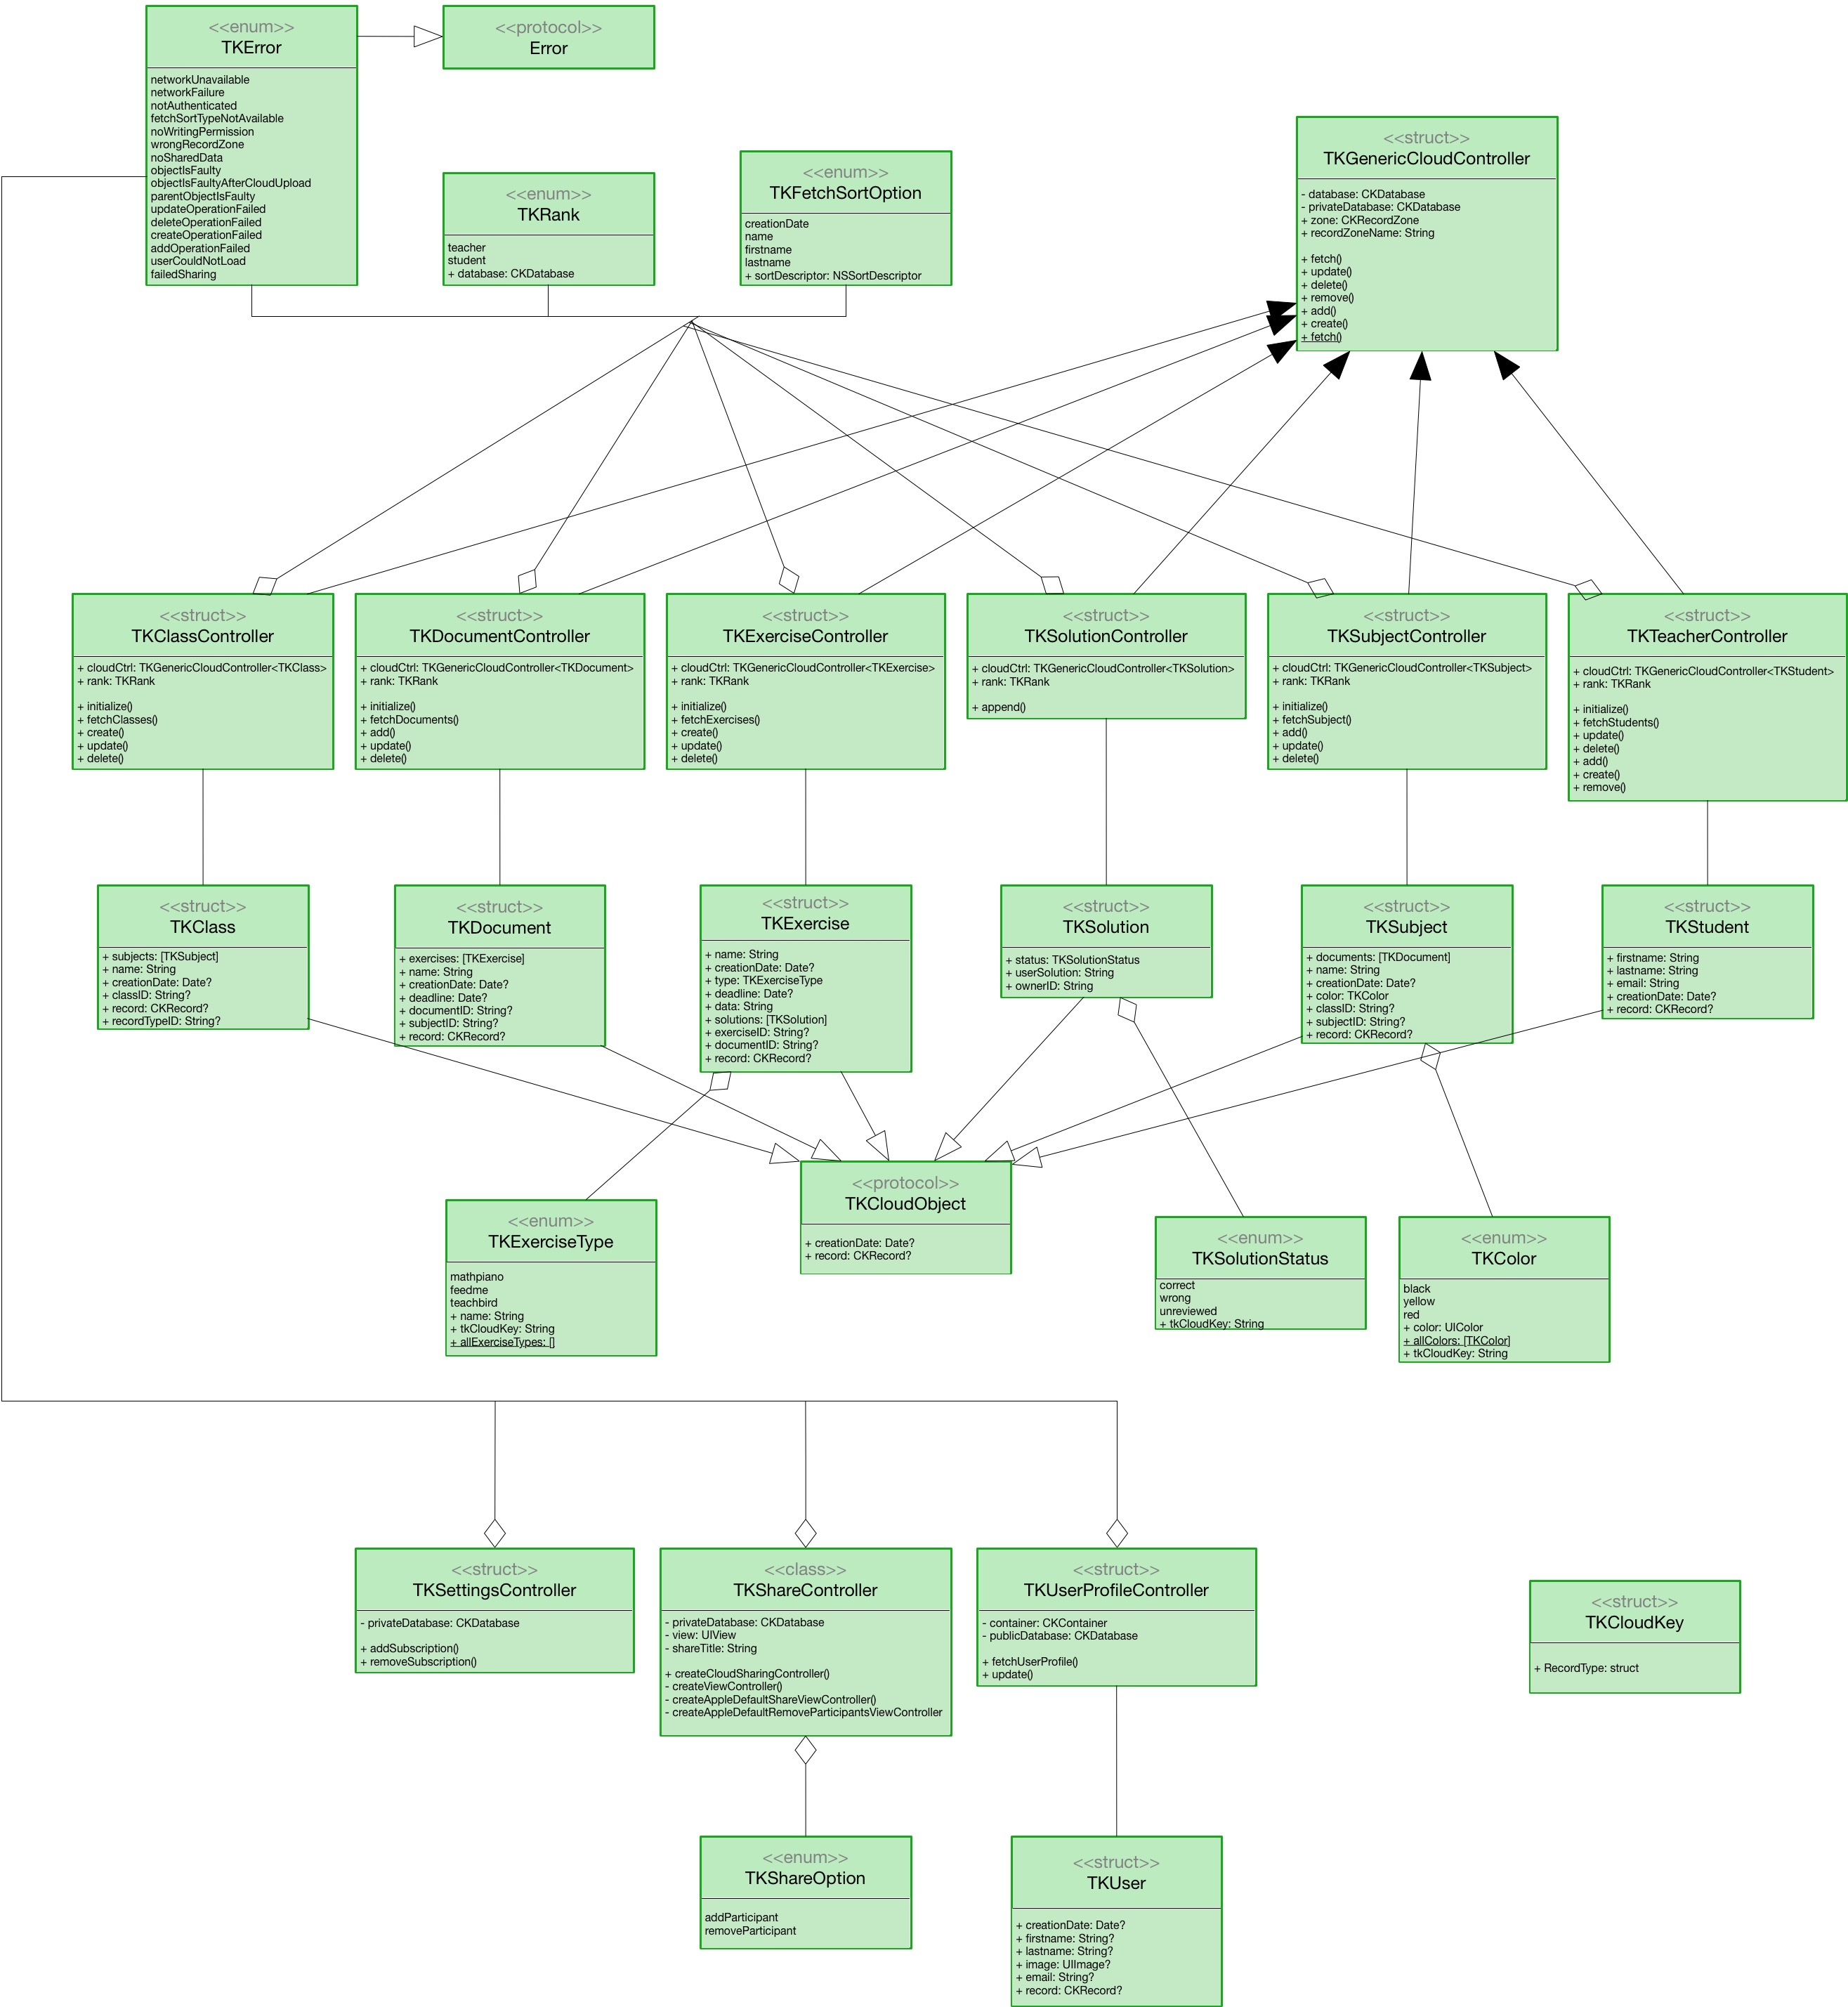
\includegraphics[width=\linewidth]{images/Klassendiagram_TeachKit.jpg}
  \caption{TeachKit Schnittstellen Klassendiagramm}
  \label{fig:diagramTeachKit}
\end{figure}

Auch TeachKit ist strikt nach der Model-View-Controller - Architektur aufgebaut. Hierbei erben alle Models, die in der Cloud gespeichert werden, von ihrer Superklasse TKCloudObject. Die Controller die diese Models verwalten, sind mit Hilfe eines generischen Controllers TKGenericCloudController implementiert worden. Alle Cloud-Models und Controller bedienen sich von verschiedenen Enumerations, die die Funktionalität übersichtlicher gestalten.

\newpage


\section{Features}

\subsection{Upload/Download/Delete/Fetch/Update}

Für jeden Datentyp in TeachKit, gibt es einen Controller der für die Operationen auf den Datentyp verantwortlich ist.
Somit gibt es folgende Controller für die Datentypen:

\begin{itemize}

\item TKClassController
\item TKSubjectController
\item TKDocumentController
\item TKExerciseController
\item TKSolutionController

\end{itemize}

Alle Controller sind ähnlich aufgebaut. Der Grund weshalb der Controller über die Methode initialize(…) funktionsfähig gemacht werden muss ist der, dass der Student auf die Shared-Database zugreift und diese zuerst gefetched werden muss.

Um doppelten Code zu vermeiden, arbeiten alle der oben genannten Controller mit dem TKGenericCloudController, der die Grundfunktionen übernimmt und in den jeweiligen Controllern dann spezialisiert werden.

\subsection{User Profile}

Zu jedem Nutzer kann der Vorname, Nachname und ein Profilbild gespeichert werden. Der TKUserProfileController der für die Nutzerverwaltung verantwortlich ist, arbeitet auf der Public-Database. Das bedeutet, dass alle Nutzer diese Informationen sehen können. Die aktuelle implementation erlaubt nur den download der Daten für den derzeit eingeloggten Nutzer. Diese kann erweitert werden, hätte aber momentan keine Verwendung gefunden.

\newpage

\subsection{Sharing}

Eines der wichtigsten Features unserer App ist das Teilen von Daten zwischen Teacher und Student. Nach dem Teilen gemeinsamer Daten haben beide Zugriff auf das Subject und alles was darunter angelegt ist.

CloudKit arbeitet mit drei verschiedenen Datenbanken.


\textbf{Private-Database}
\newline
Der aktuell angemeldete Nutzer ist der Inhaber der Daten, nur dieser hat Zugriff auf diese Datenbank und hat das Recht zu lesen und zu schreiben.
\newline
\textbf{Shared-Database}
\newline
Der aktuelle Nutzer ist nicht der Besitzer der geteilten Daten, und hat die beim Teilen zugewiesenen lese und/oder schreib Rechte.
\newline
\textbf{Public-Database}
\newline
Der aktuelle Nutzer ist nicht der Besitzer der geteilten Daten, und hat die beim Teilen Jeder App Nutzer hat lese Recht auf diese Daten, auch ohne aktiven iCloud Account.
\newline

Legt der Teacher seine Daten an, befinden diese sich in seiner private-Database. Nachdem dieser das Subject geteilt hat, befindet sich dies immer noch in der private-Database. Bei jedem Student der nun berechtigt ist, das geteilte Subject einzusehen, wird eine Referenz in der shared-Database gespeichert. Diese Referenz zeigt auf die Daten des Teachers in der private-Database.

Der Teacher teilt mit dem Student ein Subject, damit der Student die neue Arbeitsblätter einsehen kann. Mit dem Student wird der Zugriff auf Class nicht geteilt, weil er diese Information nicht benötigt.

\begin{center}
   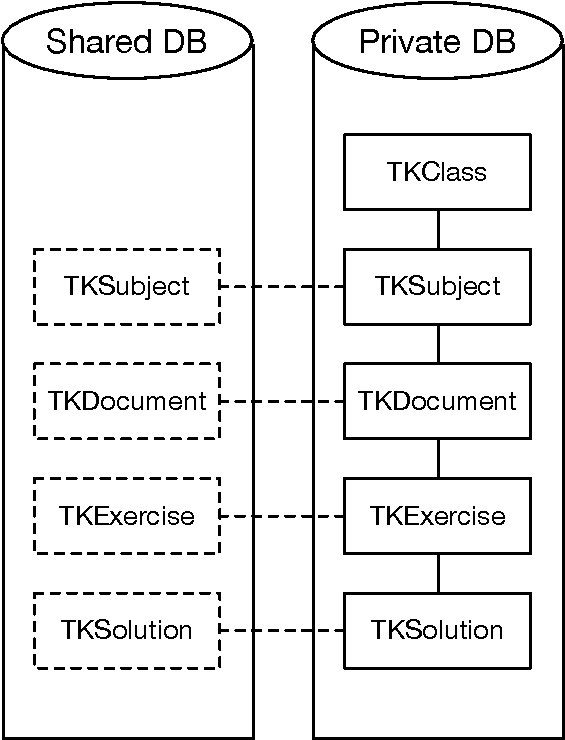
\includegraphics[width=5cm]{sharedDB_privateDB.pdf}
   \captionof{figure}{hared DB / Private DB}
\end{center}

Das Teilen findet über den TKShareController statt. Mit der Methode createCloudSharingController(…), wird der ViewController der für das Teilen verantwortlich ist erstellt und kann angezeigt werden.
Bei der Verwendung des Controllers müssen keine weiteren Bedingungen beachtet werden, der Controller kümmert sich um alles was zum Teilen benötigt wird.

\subsection{Push/Subscriptions}

Eine Besonderheit des CloudKits ist die einfache Implementierung von Push Benachrichtigungen bei Datenbankänderungen. PushNotifications in einer App zu implementieren, die über einen eigenen Server laufen, setzen PHP Kenntnisse voraus und können einiges an Zeit in Anspruch nehmen.
CloudKit Subscriptions sind jedoch einfacher zu implementieren und können auf Insert, Update, Delete und Create in der Datenbank reagieren.

Der Verwendungszweck der Subscriptions war dafür gedacht, dass der Student über Änderungen zu seinem Fach informiert wird. Dies könnte beispielsweise der Fall sein, wenn der Professor ein neues Arbeitsblatt seinem Fach hinzufügt.

Wir implementierten die CloudKit Subscriptions, die darauf reagiert, wenn der Teacher ein neues Document einem Subject hinzufügt.
Die ersten Tests auf zwei unterschiedlichen Geräten mit der gleichen Apple ID waren erfolgreich. Beim Testen über zwei unterschiedliche Apple ID’s, bei dem der Teacher ein Subject mit dem Student teilt, kamen wir allerdings an unsere Grenzen. Der Student wurde beim Hinzufügen eines neuen Objekts nicht benachrichtigt.
In der CloudKit API wurden wir dann auf die folgende Anmerkung aufmerksam, die besagt, dass Subscriptions auf der Shared-Database nicht unterstützt werden.

\newpage

\subsection{TKError}

Bei den meisten Aktionen die innerhalb des TeachKits Fehler auslösen können, werden Fehler vom Datentyp TKError erstellt. Jeder Fehler beinhaltet eine genauere Beschreibung des aufgetretene Problems. Folgende Fehler existieren:

\textbf{networkUnavailable}
Es besteht keine Internetverbindung.

\textbf{networkFailure}
Es besteht eine Internetverbindung, es konnte allerdings keine Verbindung zur Cloud hergestellt werden.

\textbf{wrongRecordZone}
Die Operation wird auf der falschen RecordZone ausgeführt oder existiert nicht. An Schnittstelle wenden.

\textbf{failedSharing}
Das Objekt konnte nicht geteilt werden.

\textbf{parentObjectIsFaulty}
Operation konnte nicht ausgeführt werden, da das Parent-Objekt Fehlerhaft ist.

\textbf{objectIsFaulty}
Operation konnte nicht ausgeführt werden, da das Objekt Fehlerhaft ist.

\textbf{objectIsFaultyAfterCloudUpload}
Auf dem Objekt wurde eine Operation in der Cloud ausgeführt. Das von der Cloud erhaltene Objekt ist inkonsistent.

\textbf{userCouldNotLoad}
Beim Zugriff auf die Nutzer Informationen ist ein Fehler unterlaufen.

\textbf{updateOperationFailed}
Der Datensatz konnte nicht geupdated werden.

\textbf{deleteOperationFailed}
Der Datensatz konnte nicht gelöscht werden.

\textbf{createOperationFailed}
Der Datensatz konnte nicht erstellt werden.

\textbf{addOperationFailed}
Der Datensatz konnte nicht hinzugefügt werden.

\textbf{fetchSortTypeNotAvailable}
Das Attribut nach dem sortiert werden soll existiert nicht.

\textbf{noWritePermission}
Der Nutzer hat keine Berechtigung die Daten zu ändern.

\textbf{noSharedData}
Die Operation konnte nicht ausgeführt werden, da noch keine Daten geteilt werden.

\newpage

\section{Aufgetretene Probleme}

\subsection{Subscription}
Da auf das Problem mit den Subscriptions bereits im Abschnitt Push/Subscriptions eingegangen wurde, erwähnen wir an dieser Stelle nur noch einmal, das Subscriptions nicht auf der Shared-Database unterstützt werden.


\subsection{Sharing}
Während der Implementation der Sharing Funktion, hatten wir über einen längeren Zeitraum das Problem, dass das Record zwischen den Nutzern geteilt wurde. Der darunter hängende Baum war allerdings nicht beim Student einzusehen.

\begin{center}
   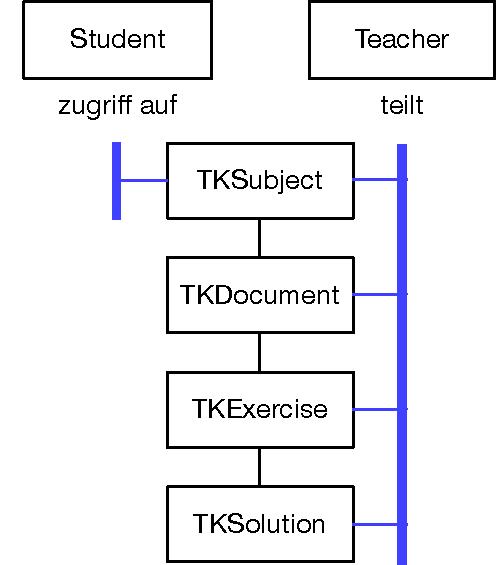
\includegraphics[width=5cm]{images/problemImage.pdf}
   \captionof{figure}{Zugriff Teacher/Student}
\end{center}

Letztendlich stellte sich heraus, dass die Verbindung zwischen Parent- und dem Child-Record nicht hergestellt wurde. Dieses Problem konnte ganz einfach mit der Methode setParent(CKRecord?) gelöst werden, allerdings musste man dafür erst wissen, dass so eine Funktion überhaupt existiert.

\newpage

\subsection{TKSolution}

Die Idee hinter TKSolution war die, dass ein Student seine Lösung darin erstellt und anschließend zu der TKExercise hinzufügt. Allerdings ist es dem Student nicht möglich, weitere Records in der geteilten Datenbank des Teachers zu erstellen und hinzuzufügen.

\begin{center}
   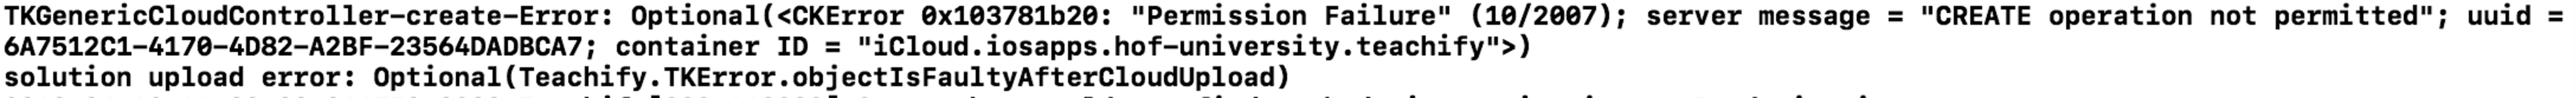
\includegraphics[width=15cm]{images/code_error.pdf}
   \captionof{figure}{Error}
\end{center}

Da diese Fehlermeldung auftritt obwohl wir die publicPermission des CKShare Objektes richtig gesetzt haben und immer noch kein Record erzeugen konnten, mussten wir eine andere Lösung dafür suchen. Wir entschlossen uns die Lösungen in ein Data-Objekt zu serialisieren und diese in TKExercise hinzuzufügen. 
Unseren neuen Lösungsansatz testen wir zuerst mit einem Attribut vom Datentyp String und nicht den eigentlich benötigten Datentyp Data. Beim ersten Upload in die iCloud werden die Records in der Cloud automatisch angelegt. Der erste Test hat geklappt und anschließend wollten wir unseren benötigten Daten vom Typ Data sichern. Da allerdings die angelegten Constraints nicht mehr für den neuen Datentyp gestimmt haben, konnten keine Records mehr hochgeladen werden. Die Constraints müssen zuerst im iCloud-Dashboard gelöscht und erneut hochgeladen werden.

